\documentclass{article}

% Cabecera del documento
% ======================================================================

% Paquetes extras
\usepackage[square, numbers, sort]{natbib}
% \usepackage{cite}
\usepackage{graphicx}
\usepackage[utf8]{inputenc}
\usepackage{amsmath,amssymb,amsfonts}
\usepackage{algorithmic}
\usepackage{textcomp}
\usepackage{subfig}
\usepackage{float}
\usepackage{mathtools}
\usepackage[spanish]{babel}
\usepackage[paper=a4paper,margin=2.75cm]{geometry}
\usepackage{booktabs} % for tables
\usepackage[colorlinks = true,
            linkcolor = blue,
            urlcolor  = blue,
            citecolor = orange,
            anchorcolor = blue]{hyperref} % for hyperlinks
\usepackage{xcolor} % text colors
\usepackage{minted}

% Directorio con imagenes
\graphicspath{{./figs/}}

% Cabecera del documento
% ======================================================================

% Titulo
\title{CONTROL DE LA PRIMER ARTICULACIÓN
DE ROBOT KR 10 R1100 sixx}

% Autores
\author{Rodrigo Pérez \\ rodrigoperez2110@gmail.com \\ \\ Control y Sistemas, Facultad de Ingeniería, \\ Universidad Nacional de Cuyo, \\ Mendoza, Argentina}

% Fecha
\date{Junio de 2023}

% Cuerpo del documento
% ======================================================================
\begin{document}

% Comandos definidos por el autor
\renewcommand{\tablename}{Tabla}
% \renewcommand{\color{blue}{#1}}{\azul}

% Crear cabecera
\maketitle

% Resumen
% ======================================================================
% \begin{abstract}
%     El presente documento presenta los contenidos mínimos que debe tener el proyecto final de la cátedra de Control y Sistemas de la Universidad Nacional de Cuyo. Además, se aclara el estilo de redacción que debe tener el informe del proyecto final y se facilitan algunos recursos para la edición de documentos en \LaTeX.
% \end{abstract}

% Secciones
% ======================================================================
\section{OBJETIVO}
\label{sec:intro}

% En la sección \ref{sec:intro}...

El presente proyecto tiene como objetivo diseñar y desarrollar el control de posición para el accionamiento electromecánico de la primer articulación del robot Kuka KR 10 R1100 sixx. El resultado esperado es lograr manipular correctamente la dinámica del robot, de forma tal que se obtenga a cada instante de tiempo la posición angular deseada de la primera articulación del mismo. Y lograrlo para cualquiera de los posibles valores de torque externo de carga mecánica del robot.


\begin{figure}[H]
    \centering
    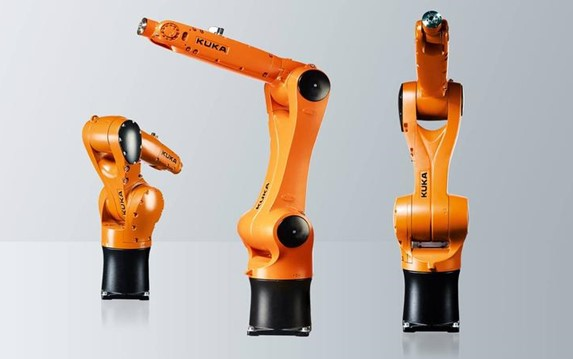
\includegraphics[width=0.75\textwidth]{3RobotsKuka}
    \caption{Robot Kuka KR 10 R1100 sixx}
    \label{fig:3RobotsKuka}
\end{figure}


% ======================================================================
\section{DESCRIPCIÓN}
\label{sec:descripciión}


\subsection{Procesamiento de señales}
\label{sec:dsp}

Un sistema mecatrónico cuenta con señales de salida, las cuales son capturadas a través del uso de sensores. Dichos sensores distan de ser perfectos, por lo que siempre introducen ruido a la señal física que se trata de medir. Ejemplos de estos sensores son giróscopos, acelerómetros, encoders, sensores ultrasónicos, entre otros.

Entonces, el proyecto propuesto debe:

\begin{enumerate}

    \item Simular las imperfecciones de los sensores de salida al agregar ruido a las señales que se obtienen a la salida del modelo.

    \item La o las salidas del sistema deben ser ruidosas. El nivel de ruido debe estar en función de la hoja de datos de un sensor real.
    % \item El nivel del ruido debe replicar el de algún sensor real, según lo que conste en la hoja de datos provista por el fabricante del sensor.
\end{enumerate}

% ======================================================================
\subsection{Modelo de la planta}
\label{sec:modelo}

A continuación, se exponen las características básicas que debe tener el modelo de la planta:

\begin{enumerate}

    \item Se deben presentar las ecuaciones que representan el modelo matemático de la planta elegida. En caso de haber desarrollado el modelo en SimScape \cite{Simscape2019}, se debe describir detalladamente el proceso de diseño.

    \item Se debe precisar si el modelo es lineal o no lineal, y si ha sido necesario linealizarlo para su control.

    \item Es importante discutir al final de esta sección cuál es el alcance y las limitaciones del modelo propuesto.

\end{enumerate}

% ======================================================================
\subsection{Controlador}
\label{sec:controlador}

El controlador debe describirse con al menos las siguientes características:

\begin{enumerate}

    \item En la gran mayoría de las aplicaciones reales el controlador es digital. Por tanto, se debe modelar un controlador discreto (PID, control en espacio de estados, etc.)

    \item Si el controlador es en espacio de estados, debe agregar un observador al sistema.

    \item Se deben especificar cuáles son los objetivos del controlador. Por ejemplo, proveer estabilidad, una respuesta rápida o una respuesta subamortiguada, entre otros posibles objetivos.

    \item Se debe hacer un análisis de observabilidad.

    \item Se debe hacer un análisis de controlabilidad.

    \item Es necesario incluir un exhaustivo análisis de perturbaciones al sistema completo, el cual incluye el modelo de planta más el controlador.

\end{enumerate}
% ======================================================================
\section{Redacción de un reporte técnico}
\label{sec:reporte-tecnico}

En la presenta sección de tratará de mostrar cómo se debe redactar un reporte técnico. El mismo debe contar con diferentes secciones, algunas obligatorias y otras opcionales. Generalmente, las primeras deben estar numeradas y las segundas, no.

\subsection{Sección de un reporte técnico}
\label{sec:secciones}

\subsubsection{Secciones obligatorias}

A continuación se detallan las secciones obligatorias.

\begin{enumerate}

    \item \textbf{Titulo}, debe ser conciso y describir brevemente el objeto de estudio del proyecto en no más de 200 caracteres.

    \item \textbf{Resumen}, también conocida como \textit{Abstract}. Su fin es el de captar la atención del lector para que lea el reporte completo. En no más de 250 palabras se debe introducir el objetivo del proyecto, justificar su desarrollo y comentar brevemente los resultados obtenidos.

    \item \textbf{Introducción}. En esta sección se justifica la importancia del proyecto desarrollado. Se plantean los objetivos del proyecto, principal y secundarios. Opcionalmente se puede describir el estado del arte del tema, esto es, qué desarrollos existen en la literatura previa y qué enfoque novedoso propone el proyecto.

    \item \textbf{Desarrollo}. Se describe la metodología utilizada para desarrollar el proyecto y las herramientas utilizadas. A su vez se puede dividir en subsecciones. En esta sección se detallan las ecuaciones del modelo de la planta y las que describen el controlador elegido. Además, se detalla el método elegido para procesar la señal ruidosa proveniente del sensor de salida de la planta.

    \item \textbf{Resultados}, se exponen los experimentos llevados adelante. Se muestran tablas y gráficos con los valores obtenidos. Se debe dar una discusión respecto a si los resultados están dentro de los valores esperados. Se agrega al sistema una señal de perturbación y se evalúa su respuesta.

    \item \textbf{Conclusiones}, expone un resumen conciso del proyecto desarrollado y de los resultados encontrados. Se discute si se cumplió con los objetivos propuestos. Adicionalmente, se puede comentar qué aspectos del proyecto se seguirán desarrollando a futuro.

    \item \textbf{Referencias}, detalla las fuentes publicadas en la literatura existente que han sido citadas durante el texto, como artículos científicos, sitios web o filminas de clase. Las referencias deben seguir un estilo de referencias, el cual se trata en la sección \ref{sec:referencias}. Esta sección no debe estar numerada.

\end{enumerate}

\subsubsection{Secciones optativas}

Entre las secciones optativas se encuentran las siguientes.

\begin{enumerate}

    \item \textbf{Bibliografía}, toda fuente de información utilizada como soporte del informe pero que no ha sido citada durante el texto. Puede incluir libros, sitios webs, videos en línea, etc.

    \item \textbf{Agradecimientos}. Lista de personas o instituciones que han ayudado o contribuido financieramente al desarrollo del proyecto y/o del informe.

    \item \textbf{Apéndices}. Material adicional que es importante agregar para dar un acabado entendimiento del reporte. Por ejemplo, código fuente, planos mecánicos o especificaciones de sensores.

\end{enumerate}

% ======================================================================
\section{Estilo del documento}
\label{sec:estilo}

El estilo propuesto para la redacción de informes técnicos está basado en el estilo de \LaTeX{} plano, sin ningún tipo de agregados. Este es el estilo que se ha elegido para la redacción de este documento.

Algunas generalidades:

\begin{enumerate}

    \item Se debe evitar hablar en primera personal del plural o ``nosotros'', ya que el informe es individual. Se debe usar voz pasiva o tercera persona del singular, por ejemplo, ``Se realizaron las siguientes actividades'' o ``Las siguientes actividades fueron realizadas''.

    \item Se debe evitar el subrayado de texto o usar negritas. Si se quiere destacar un párrafo, el mismo debe comenzar con frases como ``Cabe destacar'' o ``Es importante mencionar'', entre otras.

\end{enumerate}

En las siguientes secciones se detallan algunos aspectos de estilo que el reporte técnico debe respetar.

% ----------------------------------------------------------------------
\subsection{Información del autor}
\label{sec:autores}

Bajo el título del documento debe constar la siguiente información del autor del documento:

\begin{enumerate}
 \item Nombre completo.
 \item Dirección de e-mail.
 \item Afiliación (grupo de investigación, universidad, empresa).
\end{enumerate}

% ----------------------------------------------------------------------
\subsection{Páginas}
\label{sec:paginas}

\begin{enumerate}

    \item Todas las paginas del informe deben estar numeradas.

    \item El ancho del margen de las páginas debe estar entre 2.5 cm y 3 cm.

    \item Se debe utilizar un solo tipo de tipografía para todo el documento, con un tamaño de 11 o 12 puntos.

    \item El reporte, en lo posible, no debe superar las 30 páginas.

\end{enumerate}

% ----------------------------------------------------------------------
\subsection{Figuras}
\label{sec:figuras}

Las figuras deben tener las siguientes características.

\begin{enumerate}

    \item Deben tener fondo blanco o claro, ya que si poseen color oscuro o negro el reporte no podrá ser impreso.

    \item Deben tener grilla (\emph {grid}).

    \item Deben tener etiquetas en los ejes que especifiquen las unidades de las señales que se representan (segundos, metros, m/s$^2$, muestras (\emph{samples}), etc.).

    \item Si se representan varias señales o trayectorias en un mismo gráfico, cada línea debe representarse con diferentes colores y/o tipos de línea (continúa, puntuada, entrecortada). Además, se debe agregar una leyenda al gráfico que especifique qué representa cada línea.

    \item Las figuras deben estar numeradas en orden de aparición.

    \item Deben tener un título al pie (\emph{\textbackslash caption}) que describa el contenido de la imagen.

    \item El tamaño de las letras que son parte del gráfico deben tener un tamaño igual o levemente menor al tamaño de las letras del título al pie.

    \item Cada figura debe tener una etiqueta (\emph{\textbackslash label}) parar poder hacer referencia a la misma en el texto.

    \item Es recomendable que las figuras tengan una resolución de al menos 300 dpi.

    \item Si se toma una imagen de un libro, sitio web o trabajo científico, se debe agregar una referencia a dicha bibliografía en el título al pie de la figura.

\end{enumerate}

La figura \ref{fig:aceleraciones} es un ejemplo de cómo debe verse una gráfica.

\begin{figure}[H]
    \centering
    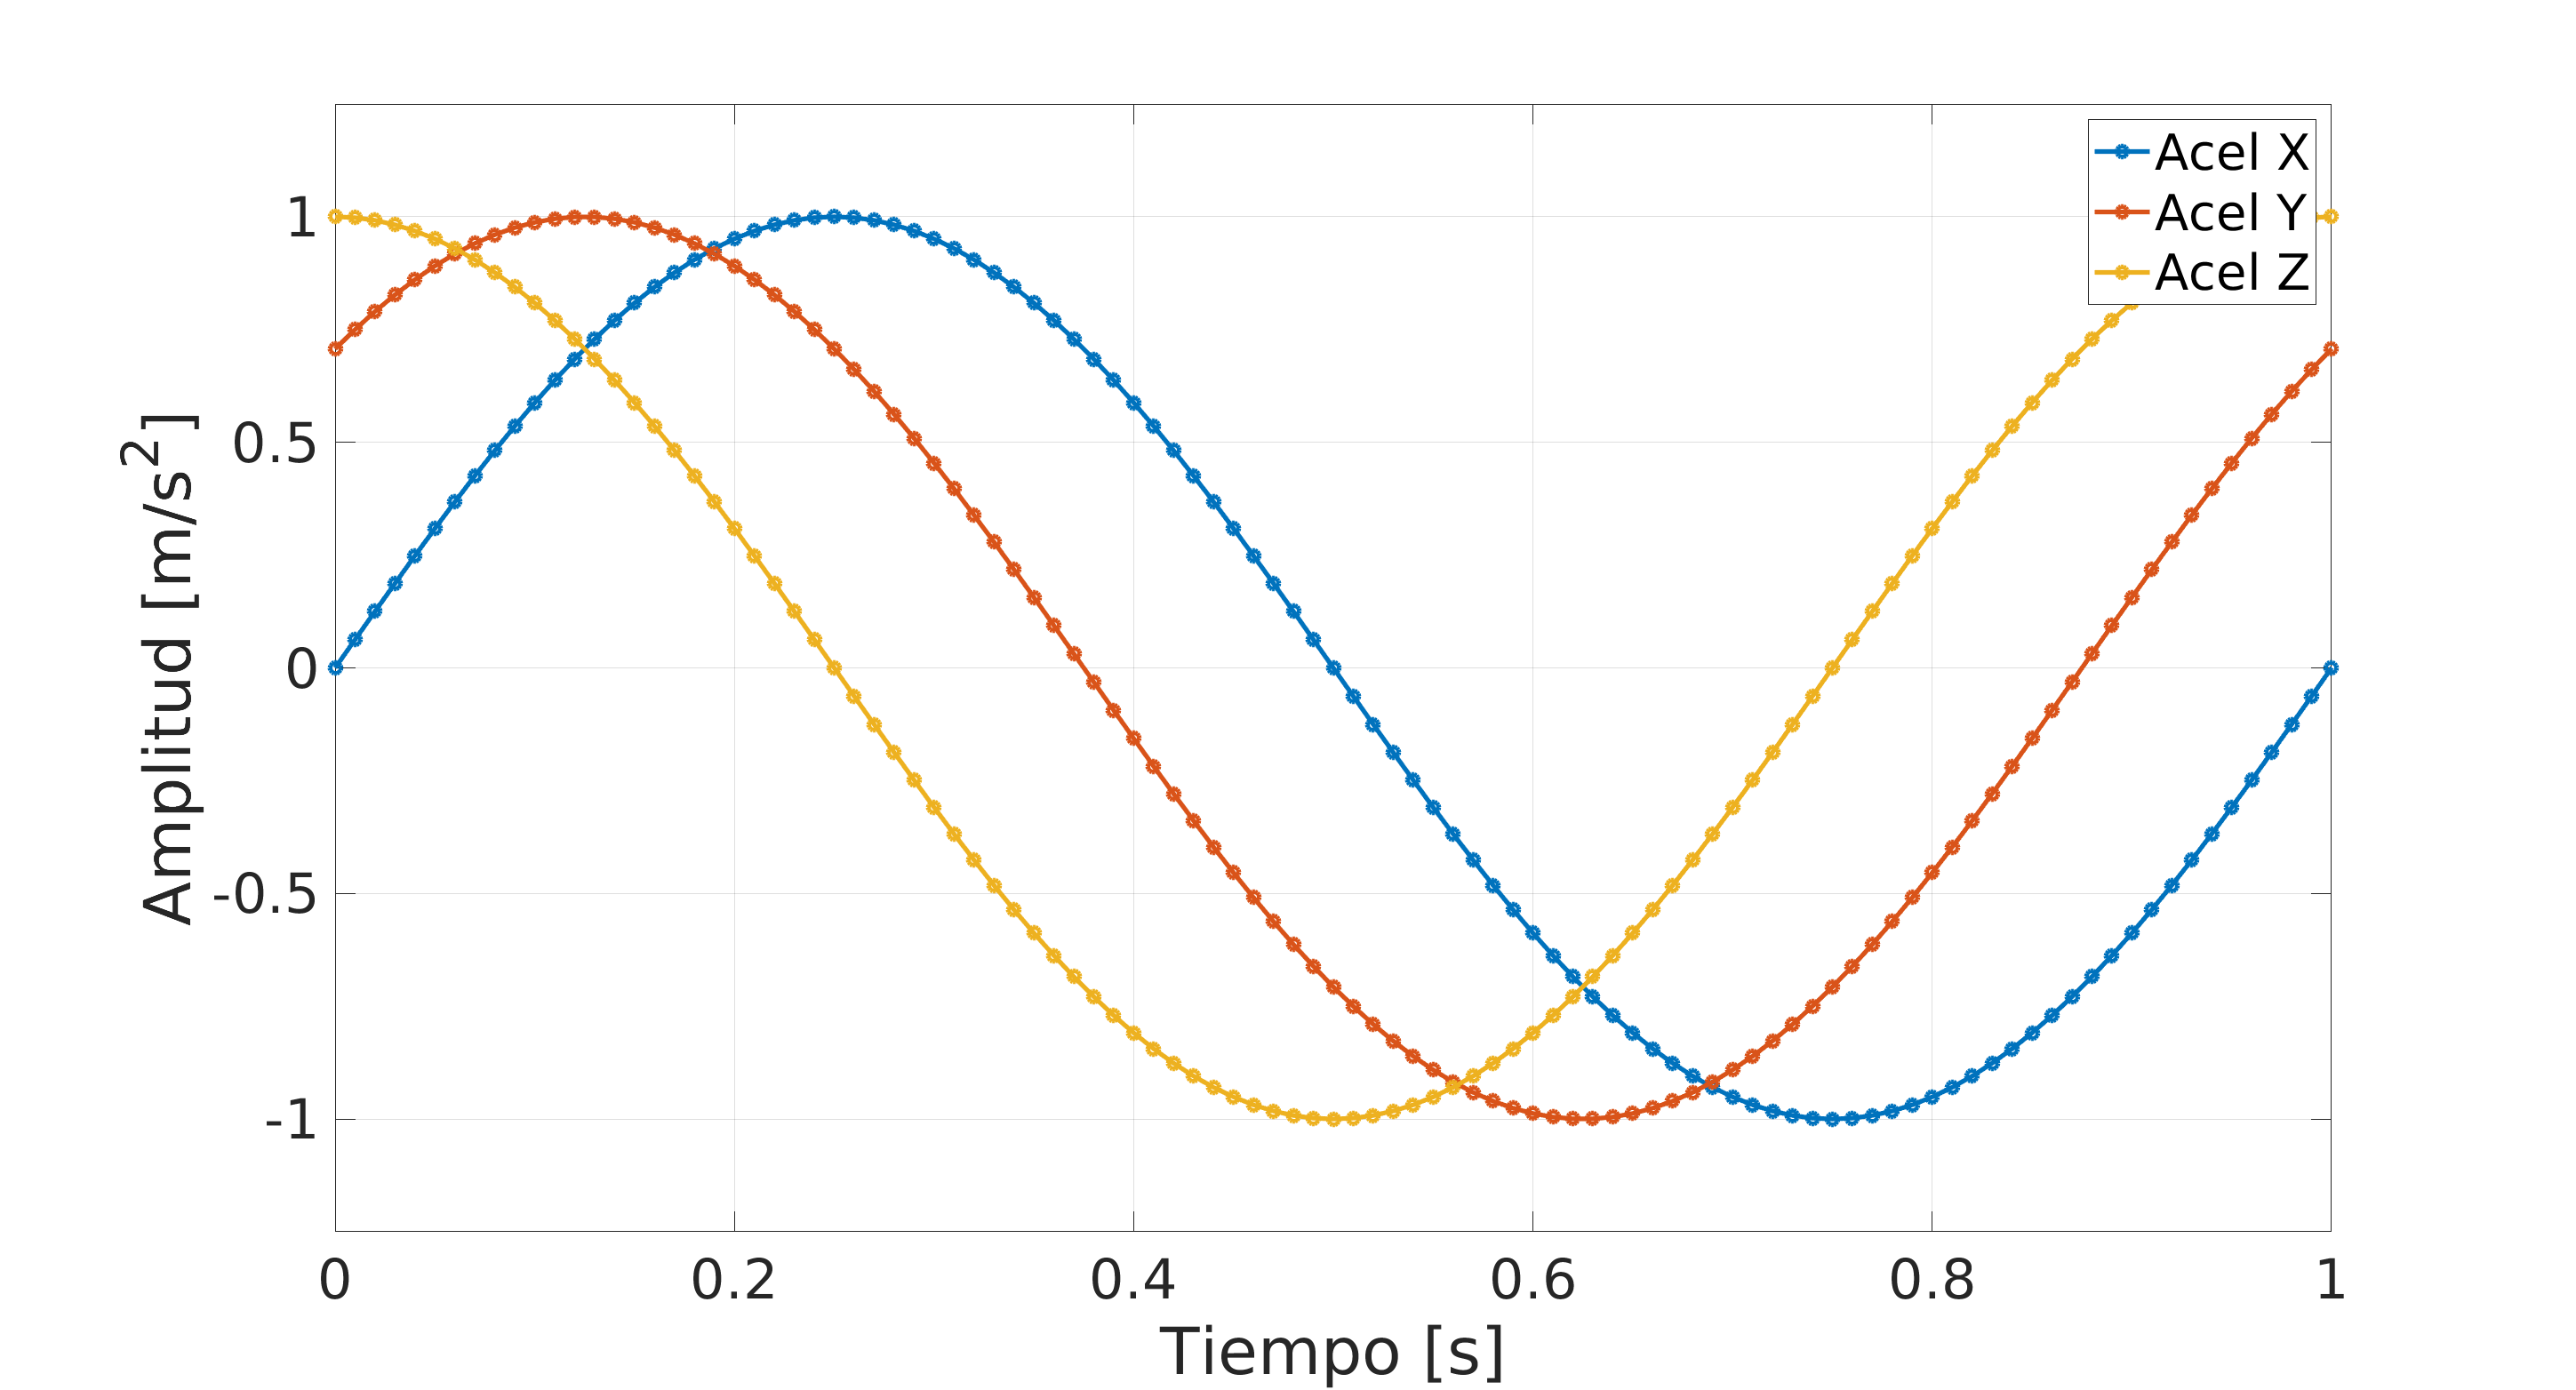
\includegraphics[width=0.75\textwidth]{aceleraciones}
    \caption{Aceleraciones (figura de ejemplo, cortesía de \cite{Gonzalez2019}).}
    % \label{fig:aceleraciones}
\end{figure}

En Apéndice se expone el código fuente en MATLAB con el que fue confeccionada la figura \ref{fig:aceleraciones}.

% ----------------------------------------------------------------------
\subsection{Tablas}
\label{sec:tablas}

Características que deben tener las tablas o cuadros en el reporte:

\begin{enumerate}

    \item Deben estar numeradas en orden de aparición.

    \item Deben tener un título (\emph{\textbackslash caption}) que describa el contenido de la tabla. Puede ubicarse arriba o al pie.

    \item Cada tabla debe tener una etiqueta (\emph{\textbackslash label}) parar poder hacer referencia a la misma durante el texto.

\end{enumerate}

La tabla \ref{tab:IMU-static} expone un ejemplo de tabla. Se ha utilizado el paquete \emph{booktabs} para obtener un acabado más profesional.

\begin{table}[ht]

\small
	\centering
	\caption{Static bias (SB) and standard deviation ($\sigma$) from static analysis of the two IMUs under study.}
	\label{tab:IMU-static}
	\begin{tabular}{l cc cc}

	\toprule %

	&  \multicolumn{2}{c}{ \textbf{Static bias} } &  \multicolumn{2}{c}{ \textbf{$\sigma$}} \\

    &  \multicolumn{2}{c}{(m$/\text{s}^2$) (rad$/$s) }   &  \multicolumn{2}{c}{(m$/\text{s}^2$) (rad$/$s) } \\

	\midrule

	&  {MPU-6000} & Ekinox &  {MPU-6000} & Ekinox \\

	\midrule

 Acc X      & -1.347\emph{e}-1  	& 1.611\emph{e}-4  	& 1.294\emph{e}-2 	& 2.293\emph{e}-3 \\

 Acc Y      & 7.202\emph{e}-2  	& 2.599\emph{e}-2  	& 1.324\emph{e}-2 	& 2.008\emph{e}-3  \\

 Acc Z     	& 9.735\emph{e}+0   	& 9.804\emph{e}+0 	& 2.012\emph{e}-2  	& 2.336\emph{e}-3 \\

 Gyro X     & -1.616\emph{e}-3 	&-2.451\emph{e}-4  	& 7.026\emph{e}-4   	& 1.023\emph{e}-2 \\

 Gyro Y  	& 1.387\emph{e}-3   	& 1.230\emph{e}-4 	& 6.325\emph{e}-4  	& 9.574\emph{e}-3 \\

 Gyro Z  	& 2.037\emph{e}-3   	& -2.216\emph{e}-5	& 6.218\emph{e}-4   	& 9.423\emph{e}-3 \\

	\bottomrule

\end{tabular}
\end{table}

Existen herramientas en línea que facilitan el armado de tablas en \LaTeX $\,$ \cite{TableGenerator}.

% ----------------------------------------------------------------------
\subsection{Ecuaciones}

Características que deben tener las ecuaciones en un reporte técnico:

\begin{enumerate}

    \item Deben estar numeradas en orden de aparición.

    \item Deben ocupar una línea por ecuación.

    \item Las ecuaciones que se representan durante el texto no deben numerarse, por ejemplo, $ \sqrt{\frac{1}{2}} $ o
    $ A = \begin{bmatrix} 1,2 \\ 3,4\\ \end{bmatrix} $. Estas ecuaciones pueden representarse en \LaTeX{} entre dos símbolos pesos (\$ ecuacion \$).

    \item Cada ecuación debe tener una etiqueta  (\emph{\textbackslash label}) parar poder hacer referencia a la misma durante el desarrollo del texto.

    \item En lo posible no se deben agregar ecuaciones como imágenes.

\end{enumerate}

A continuación algunos ejemplos de ecuaciones. Las ecuaciones \ref{eq:cbn} se agrupan en un sólo número de ecuaciones, pero a su vez se pueden referenciar por separado como ecuación \ref{eq:omega} y ecuación \ref{eq:deltaPsi}.

\begin{subequations} \label{eq:cbn}
	\begin{align}
		\label{eq:omega}    C^n_{b(+)} &= C^n_{b} (I + {\delta \Psi})  \, , \\
		\label{eq:deltaPsi} \delta \Psi &= [ {\delta \boldsymbol e} \, \times ] \, .
	\end{align}
\end{subequations}

\begin{align} \label{eq:limite}
\lim_{ \delta t \to 0} {\frac {\delta \Psi }{\delta t }} = {\Omega_{nb}^b} \, .
\end{align}

\begin{subequations} \label{eq:inc_psi}
	\begin{align}
	 C_{b}^{nT} C_{b(+)}^n  &= \overbrace{ C_{b}^{nT} C_{b}^n}^{I} ( I + {\delta \Psi} )  \, , \\
	 \implies {\delta \Psi} &= C_{b}^{nT} C_{b(+)}^n - I  \, , \\
							&= C_{n}^b    C_{n(+)}^{bT} - I \, .
	\end{align}
\end{subequations}

\begin{align} \label{eq:vrw}
	{\boldsymbol n}_f &= \frac{ \text{VRW} }{60} \left ( \frac{\text{m/s}^2}{\sqrt{\text{Hz}}} \right ) \, .
\end{align}

\begin{subequations}  \label{ned2ecef}
	\begin{align}
		\label{eq:pe}{\boldsymbol p}^e &= {\boldsymbol p}^e_{o} + R^e ~ {\boldsymbol p}  \, , \\
		R^e &=
		\begin{bmatrix}
			-\sin {\gamma_o} \cos {\lambda_o} & -\sin \lambda_o & -\cos \gamma_o \cos \lambda_o \\
			-\sin {\gamma_o} \sin {\lambda_o} &  \cos \lambda_o & -\cos \gamma_o \sin \lambda_o \\
			 \cos {\gamma_o}		  & 0	            & -\sin \gamma_o
		\end{bmatrix} \, .
	\end{align}
\end{subequations}

\begin{align}
\label{eq:h-matrix} H_{\{6\times21\}} =
\begin{bmatrix}
        \boldsymbol{0} & I  & \boldsymbol{0} &\boldsymbol{0}& \boldsymbol{0} &\boldsymbol{0}& \boldsymbol{0} \\
        \boldsymbol{0} & \boldsymbol{0} & ~\hat T_p^r  &\boldsymbol{0}& \boldsymbol{0} &\boldsymbol{0}& \boldsymbol{0}\\
  \end{bmatrix} \, .
\end{align}

% ----------------------------------------------------------------------
\subsection{Referencias} \label{sec:referencias}

El sistema de referencias en \LaTeX{} es muy versátil pero a su vez tiene ciertas particularidades.

Las referencias se guardan en texto plano en un archivo con extensión .bib en formato BibTex. Existen distintos tipos de citas, según el tipo de documento al que se quiera hacer referencia (artículo en congreso, en revista, libros, manuales, etc.). En \cite{BibtexExamples2019} se pueden ver todas las variantes que ofrece el formato BibTex.

Por otra parte, existen varios formatos para incluir citas en un documento. Pueden usarse números entre corchetes, por ejemplo [15], o apellido del autor y año de publicación, por ejemplo (Pérez, 2011). En general, en los reportes técnicos se suele usar el primer formato, el mismo que se utiliza en este documento. Por otra parte, las referencias pueden numerarse por orden alfabético o por orden de aparición.

En general, una referencia debe tener la siguiente estructura:

[1] Nombre del autor. Título de la obra. Donde fue publicado (Conferencia, Revista, Editorial). Lugar de publicación, Fecha de publicación.

% ======================================================================
\section{Anglisismo y neologísmos}

El proyecto final de la cátedra puede ser escrito en español o en inglés. Si se elige escribirlo en español, se deben tomar algunos recaudos para que el documento no se transforme en una mala mezcla de ambos idiomas.

En general se debe evitar el \emph{spanglish}, esto es, abusar del uso de palabras en inglés. No se deben usar palabras en inglés que poseen una traducción unívoca en español. Un ejemplo de esto puede ser la palabra en inglés \emph{performance}, cuya traducción es desempeño o rendimiento. La Real Academia Española provee un listado de palabras técnicas en inglés y su traducción al español \cite{Rae2019}.

Por otro lado, a veces es conveniente usar palabras en inglés que tienen un uso muy difundido y cuya traducción no deja en claro de qué se está hablando. Ejemplos de esto pueden ser las palabras \emph{hardware}, \emph{software} o \emph{router}.

Otro aspecto a tener en cuenta es el correcto uso de los gerundios en español, cuyo uso difiere del que se hace en el inglés \cite{Mandado}.

% ======================================================================
\section{Diseño de documentos en \LaTeX}

Existe mucha documentación en Internet para aprender a diseñar un documento en \LaTeX. Un buen punto de partida puede ser \cite{Latexbook}.

Respecto a las herramientas para crear documentos en \LaTeX{}, hay varias opciones. Tal vez la opción más práctica es usar Overleaf.com \cite{Overleaf2019}. Este sitio es gratuito y pone a disposición de sus usuarios una interfaz web para la creación de documentos en \LaTeX. Además, permite exportar el documento en formato pdf.

El presente documento puede ser tomado como un ejemplo de diseño en \LaTeX{} a través del link a Overleaf.com provisto en \cite{Gonzalez2019}.

% ======================================================================
% Seccion sin numeracion

\section*{Bibliografía}

Wikibooks. Online \LaTeX{} book. \href{https://en.wikibooks.org/wiki/LaTeX/}{https://en.wikibooks.org/wiki/LaTeX/}.

Overleaf. Learn LaTeX in 30 minutes. \href{https://www.overleaf.com/learn/latex/Learn_LaTeX_in_30_minutes}{URL}.

Overleaf. Bibliography management in LaTeX. \href{https://www.overleaf.com/learn/latex/Bibliography_management_in_LaTeX}{URL}.


% Referencias
% ======================================================================

% Estilo de citas
\bibliographystyle{unsrt}

% Nombre del archivo .bib
\bibliography{references}

% ======================================================================
% Seccion sin numeracion

\section*{Apéndice}

A continuación, se expone el código fuente en MATLAB con el que se confeccionó la figura \ref{fig:aceleraciones}.

\inputminted{matlab}{figura_ejemplo.m}

\end{document}
